%===============================================================================
%      Le boot
%===============================================================================
\section{Le boot}

   Nous allons ici voir comment en arriver à un noyau présent dans la
mémoire de la machine, prêt à être exécuté. Nous décrirons deux pistes

\begin{itemize}
   \item Nous commencerons par nous fonder sur une situation ``à
     l'ancienne'' avec un \textsc{pc} doté d'un lecteur de
     disquettes. Nous utiliserons alors le  \textsc{bios} du \textsc{ pc}
     pour charger le noyau en mémoire, lui passer quelques
     informations et le faire démarrer.

   \item Nous observerons ensuite des outils un peu plus modernes
     permettant de démarrer de façon un peu plus simple et plus
     indépendante du matériel sous-jacent.
  
\end{itemize}


%-------------------------------------------------------------------------------
%
%-------------------------------------------------------------------------------
\subsection{Démarage à partir d'une disquette}

   Nous allons donc devoir mettre en \oe{}uvre le boot du noyau dans
cette configuration. Pour cela, nous allons construire un fichier qui
sera placé sur une disquette à partir de laquelle notre système pourra
démarrer. Ntons que nous utiliserons ici un émulateur comme Qemu
auquel nous donnerons le chemin vers ce fichier et à qui nous
demanderons de démarrer depuis cette disquette.

   Observons la structure de ce fichier puis regardons comment en
construire chaque partie.

%-------------------------------------------------------------------------------
%
%-------------------------------------------------------------------------------
\subsection{Construction du fichier de démarrage}

   Afin de permettre un démarrage ``à l'ancienne'' par un boot sur
disquette du \textsc{ pc}, nous allons donc construire une image de disquette
dont la structure est décrite par la figure \ref{fig:image-disquette}.

\begin{figure}[htbp]
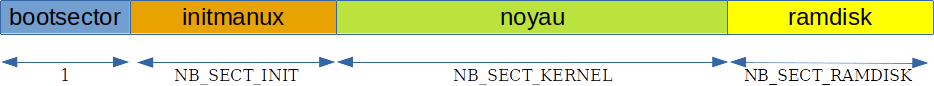
\includegraphics[width=0.8\textwidth]{image-disquette}
\caption{\label{fig:image-disquette}Le fichier de démarage}
\end{figure} 

   Ce que j'appelle ici le boot du système se passera donc en deux
temps. D'abord le secteur de boot est chargé en mémoire par le
\textsc{ bios} qui lui donne la main.

   Le secteur de boot  s'occupe alors de charger en mémoire le code
d'initialisation ainsi que le code du noyau. Il donne alors à son tour
la main à l'initialisation. Ce second élément réalise quelques
opération puis démarre enfin le noyau.

   Si le secteur de boot et le code d'initialisation sont deux
éléments distincts, c'est pour deux raisons principales

\begin{itemize}
   \item d'une part le secteur de boot ne dispose que de 512 octets,
     si bien qu'il doit être réduit au  minimum ;
   \item chacun de ces deux éléments à un rôle bien spécifique
     (charger le code en mémoire et initialiser le système).
\end{itemize}

   Avant de regarder en détail comment ils sont mis en \oe{}uvre,
regardons les interactions entre les rois éléments.
   
%-------------------------------------------------------------------------------
%
%-------------------------------------------------------------------------------
\subsection{Liens entre les trois éléments}

   Les trois parties de codes évoquées ici (le secteur de boot, le
code d'initialisation et le noyau) ne sont pas liées entre elles (par
une édition de liens). Les appels de fonction, partages de variables,
\ldots {} sont alors à éviter car peu pratiques !

   Concrètement, il y a surtout deux ``appels de fonction'' à réaliser : 

\begin{itemize}
   \item le secteur de boot doit lancer le code d'initialisation ;
   \item le code d'initialisation doit démarrer le noyau.
\end{itemize}

   Pour cela, on va utiliser le fait que tous les éléments sont
placés à des adresses connues et faire un saut à ces adresses.
   
%-------------------------------------------------------------------------------
%
%-------------------------------------------------------------------------------
\subsection{Le secteur de boot}

   Lorsqu'on allume un \textsc{ pc} normalement configuré avec une disquette dans
le premier lecteur, le \textsc{ bios} charge le premier secteur de la diquette en
mémoire et l'exécute. En fait, il ne fait cela que si les deux derniers octets
de ce secteur contien\-nent la valeur magique {\tt 0xAA55}. Pour être
plus précis, c'est à l'adresse {\tt 0x7C00} que ce secteur est chargé.

   Un secteur étant composé traditionnellement de 512 octets, on ne
peut pas faire des folies avec le secteur de boot ! On va donc se
contenter de charger en mémoire d'autres secteurs du disque. Pour
cela, on peut utiliser le \textsc{ bios} et plus particulièrement
l'interruption 13h qu'il nous fournit pour manipuler les lecteurs.

   Le secteur de boot de ManuX est codé dans le fichier
\lstinline!boot/bootsector.nasm! et il est donc écrit en NASM. Il est
très simple et se contente d'utiliser le \textsc{ bios} pour charger le
noyau en mémoire puis de faire un saut au début de la mémoire ainsi
initialisée.

   Il n'est pas très robuste, en particulier sur la taille attendue du
noyau et sur l'adresse à laquelle le placer !

   Concrètement, ce chargement se fait en deux phases :

\begin{itemize}
   \item Chargement du code d'initialisation : c'est le code qui va
     avoir pour rôle d'initialiser le système. Ce code est écrit en
     assembleur dans le fichier \lstinline!boot/init-manux.nasm!.
   \item Chargement du code du noyau : c'est tout le code de ManuX qui
     est ici chargé en mémoire. Il sera exécuté par le code
     d'initialisation. 
\end{itemize}

   Après ces deux chargements, le code du secteur de boot exécute le
code d'initialisation.

   Je ne décris pas plus ce code qui ne présente pas un intérêt
profond, les plus curieuses et curieux n'ont qu'à lire le code !
   
%-------------------------------------------------------------------------------
%
%-------------------------------------------------------------------------------
\subsection{État de la mémoire après le chargement}

   L'état de la mémoire à la fin du boot est décrite par la figure
\ref{etat-memoire-boot}.

\begin{figure}[htbp]
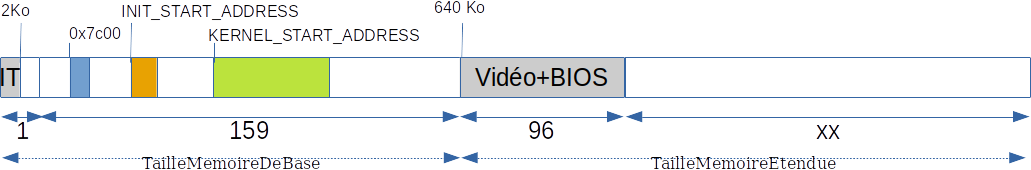
\includegraphics[width=\textwidth]{etat-memoire-boot}
\caption{\label{fig:etat-memoire-boot}État de la mémoire après le boot}
\end{figure} 

   Une fois qu'il a terminé son travail, le code du secteur de boot
donne la main au code d'initialisation.
   
%-------------------------------------------------------------------------------
%      L'initialisation
%-------------------------------------------------------------------------------
\subsection{L'initialisation}

   Le "programme" d'initialisation est traditionnellement consacré à la détection
et à l'initialisation (original, vu son nom !) du matériel. Sur un \textsc{ pc} de
base, on peut là encore se faire aider du \textsc{ bios}. 

   En ce qui concerne ManuX, cette phase d'initialisation va profiter
du fait qu'elle n'a pas les mêmes limites de taille que le secteur de
boot (un seul secteur comme le nom au singulier le suggère). On va
donc pouvoir y réaliser certaines actions un peu plus confortablement,
comme :

\begin{itemize}
   \item Vérifier la mémoire disponible (cette information sera passée au
  noyau).
   \item Charger en mémoire un ramdisk qui nous permettra de jouer avec
    des systèmes de fichiers  sans avoir besoin d'implanter la gestion
    de matériel.
\end{itemize}

   Voyons rapidement quelques points.

%...............................................................................
%      Passage des informations au noyau
%...............................................................................
\subsubsection{Passage des informations au noyau}

   La plupart des informations recueillies par l'initialisation peuvent se
révéler particulièrement intéressantes pour le noyau. Il est donc important de
se définir un mécanisme permettant de faire passer ces informations depuis la
phase d'initialisation jusqu'au noyau.

   Pour cela, nous déclarons la "fonction principale" du noyau comme prenant
en paramètre l'adresse d'une structure dans laquelle seront enregistrées ces
différentes informations. Nous aurons donc par exemple la définition suivante

\begin{lstlisting}{}
typedef struct _InfoSysteme {
   uint16 memoireDeBase;
   uint16 memoireEtendue;
   /* ... */
} InfoSysteme;
 
void _start(InfoSysteme * infoSysteme)
{
   /* ... */
}
\end{lstlisting}

   Naturellement, pour que tout cela fonctionne, il est nécessaire, à la fin
de la phase d'initialisation, d'empiler l'adresse de la structure dans laquelle
les informations ont été enregistrées. Voici donc par exemple à quoi peuvent
ressembler les dernières lignes de la phase d'initialisation :

\lstset{language=nasm}

\begin{lstlisting}{}
; Calcul de l'adresse des infos Systeme
;--------------------------------------
mov   eax, 0                   ; C'est a cette adresse que
mov   ax, MANUX_INIT_SEG_16    ; sont actuellement les infos
shl   eax, 4                   ; Il faut transformer
add   eax, InfoSysteme         ; en adresse "flat"
push  eax
 
; Et c'est parti, on saute sur le noyau !
;----------------------------------------
mov   eax, MANUX_KERNEL_SEG_16
shl   eax, 4
call  eax 
\end{lstlisting}

   Notons que, bien sûr, aucun contôle de type ne peut être fait entre les deux
phases et qu'il est donc important que le programmeur définisse de façon
cohérente la structure C et la zone mémoire gérée en assembleur.

%...............................................................................
%      Détection de la mémoire
%...............................................................................
\subsubsection{Détection de la mémoire}

%...............................................................................
%      Détection du processeur
%...............................................................................
\subsubsection{Détection du processeur}

%...............................................................................
%      
%...............................................................................
\subsubsection{Démarrage du noyau ({\tt noyau/main.c})}

   La dernière action du programme d'initalisation est donc l'exécution
de la fonction \lstinline!_start()!. Comme je l'ai dit précédemment,
il ne s'agit pas d'un appel de foncion C classique, puisque les deux
morceaux de code ne sont pas liés entre eux, mais d'un saut à
l'adresse de la fonction (le tout après avoir empilé les paramètres).

   Ceci termine donc la description de toute la quincailleire qui nous
permet d'arriver au début de l'exécution du code du noyau. Nous allons
commencer la description de ce dernier par la mise en place des outils
de base dont il aura besoin.

%-------------------------------------------------------------------------------
%
%-------------------------------------------------------------------------------
\subsection{Utilisation de {\em Multiboot}}

   Nous allons ici utiliser la spécification {\em Multiboot} définie
par la {\em Free Software Foundation} qui va nous permettre d'utiliser
les services d'outils tels que \textsc{ grub} afin de grandement simplifier
le chargement du noyau de ManuX.

   Cela nous permettra également d'utiliser des outils un peu plus
modernes qu'un lecteur de disquettes et, par voie de conséquence, de
faire fonctionner ManuX sur autre chose que des machines virtuelles ou
hors d'age !


%-------------------------------------------------------------------------------
%
%-------------------------------------------------------------------------------
\subsection{Réalisation d'une image {\sc iso}}


